\documentclass[12pt]{article}
\usepackage{fancyhdr,epsfig,graphics,tabularx,times,wrapfig}
\pagestyle{empty}
\topmargin=-0.75in
\oddsidemargin=-0.5in
\textwidth=7.5in
\textheight=10.25in
\parindent=0.0in
\parskip=10pt
\linespread{1.0}

\renewcommand{\labelenumi}{(\alph{enumi})}
\renewcommand{\thefigure}{\arabic{section}.\arabic{figure}}
\def\thesection{Problem \#\arabic{section}}

\begin{document}
{\bf BME154L - Exam \#1}\hfill Name:\underline{\hspace*{3.0in}}



\vspace*{0.5in}

\centerline{\LARGE BME154L (Palmeri)}
\vspace*{0.25in}
\centerline{\LARGE Spring 2012}
\vspace*{0.25in}
\centerline{\LARGE Exam \#1}
\vspace*{0.25in}

{\bf Instructions:} 
\begin{itemize}
\item Write your name at the top of each page.
\item Show all work (this is {\it critical} for partial credit!).
\item \underline{Remember to include units with all answers and label all plot axes.}
\item Clearly box all answers.
\item Assume that all components are ideal unless otherwise stated.
\item Assume that op amps rail at $\pm$ 12 V unless otherwise stated.
\end{itemize}

\begin{center}
\begin{tabular}{cc}
\includegraphics[width=0.39\linewidth]{avery.jpg} &
\includegraphics[width=0.3\linewidth]{ziva.jpg} \\
\end{tabular}

Avery \& Ziva wish you good luck!!
\end{center}


\emph{In keeping with the Duke Community Standard, I have neither given nor received aid in completion of this examination.}

\vspace*{0.5in}

Signature:\underline{\hspace*{3.0in}}


\clearpage

{\bf BME154L - Exam \#1}\hfill Name:\underline{\hspace*{3.0in}}



\section{[10 points]}

{\bf Input/Output Impedance (Revisited)}

Impedances can be in terms of $R$s and $C_1$.  Please don't answer the `Why?' questions below with more than 2-3 sentences!!

\begin{center}
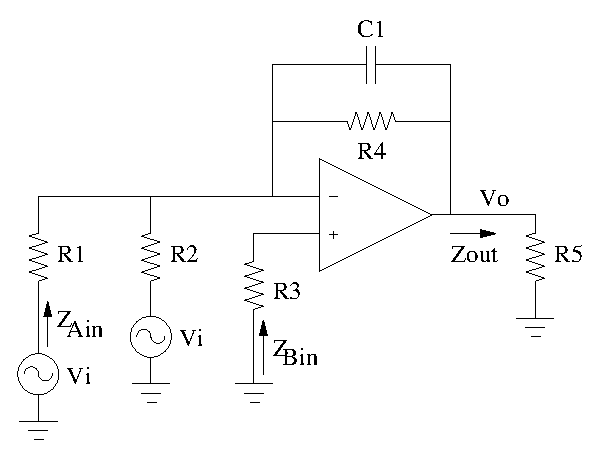
\includegraphics[width=3.0in]{zin_zout.eps}
\end{center}

\begin{enumerate}
\item What is the input impedance ($Z_{A_{in}}$), as indicated on the circuit above?
\item What is the input impedance ($Z_{B_{in}}$), as indicated on the circuit above?
\item Which input impedance is more ideal when working with voltage input signals?  Why?
\item What is the output impedance ($Z_{out}$), as indicated on the circuit above?
\item What is the ideal output impedance when working with voltage signals?  Why?
\end{enumerate}

\clearpage

{\bf BME154L - Exam \#1}\hfill Name:\underline{\hspace*{3.0in}}



\clearpage

{\bf BME154L - Exam \#1}\hfill Name:\underline{\hspace*{3.0in}}



\section{[30 points]}

{\bf Cardiovascular Anatomy/Physiology and the ECG Signal}

\begin{enumerate}
\item Today is Vivek's birthday, but he started ``pre-gaming'' this weekend
while studying for BME154 by putting ECG pads all over his body.  One of his
friends was helping him with this task, but that friend started handing him
pads without gel on them.  Vivek threw the pads down in disgust and quickly
explained why the pads needed gel to optimize their function.  What was Vivek's
explanation?  (It is okay to assume that Vivek was correct.)
\item What is the primary function of the sino-atrial (SA) node in the heart?
\item What are the two most important functions of the atrio-ventricular (AV) node in the heart?
\item The QRS complex represents what electrical process in the heart?
\item Myocardial ischemia can cause what changes to the QRS complex of the heart?  Why do these changes occur?
\item Put the following pieces of the electrical system of the heart in order
of depolarization for a heart beat, starting just before the P wave would be
present on an ECG trace:
\begin{itemize}
    \item Bundle of His
    \item Purkinje Fibers
    \item AV Node
    \item SA Node
    \item Left/Right Bundle Branch
\end{itemize}
\item High blood pressure can cause the ventricles of the heart to hypertrophy.  Please answer the following with 1-2 sentences.
\begin{enumerate}
    \item What is hypertrophy and why does this occur?
    \item How might ventricular hypertrophy be evident on an ECG trace?
    \item What does ventricular hypertrophy do to cardiac stroke volume in the extreme case (think of the over-developed bicep from lecture)?
\end{enumerate}
\item Having ECG lead wires of equal impedance reduces noise for certain
capacitive coupling problems, but not others.  In the context of capacitive
coupling to wires and the body, (1) explain which scenario benefits from equal
impedance lead wires (and why), and (2) what the ideal absolute impedance of the
wires should be in each case relative to the input impedance of the ECG monitor
they are attached to.
\end{enumerate}

\clearpage

{\bf BME154L - Exam \#1}\hfill Name:\underline{\hspace*{3.0in}}



\clearpage

{\bf BME154L - Exam \#1}\hfill Name:\underline{\hspace*{3.0in}}



\clearpage

{\bf BME154L - Exam \#1}\hfill Name:\underline{\hspace*{3.0in}}



\section{[40 points]}

{\bf Analog $\leftrightarrow$ Digital}

A 4-bit successive approximation ADC is calibrated to convert voltages ranging from 5 - 20 V.

\begin{enumerate}
\item How many discrete voltage levels can be represented by a 4-bit number?
\item What is the voltage of the least significant bit for this ADC?
\item What is the highest signal-to-noise ratio (SNR) that this ADC can
accurately convert without wasting bits on sampling noise?
\item How many voltage comparisons are made during the successive approximation
of the 4-bit number?
\item If the input voltage being converted is 17.3V, then solve for the
discrete voltages that are compared to the input voltages during this process
(list them in order of how they are compared in this ADC).  (Show your work for
this to get partial credit!)
\item This ADC is only as good as the DAC that is being used ``behind the
scenes''.  Design an R-2R DAC that can be used in this successive approximation
ADC.
\end{enumerate}

\clearpage

{\bf BME154L - Exam \#1}\hfill Name:\underline{\hspace*{3.0in}}



\clearpage

{\bf BME154L - Exam \#1}\hfill Name:\underline{\hspace*{3.0in}}



\clearpage

{\bf BME154L - Exam \#1}\hfill Name:\underline{\hspace*{3.0in}}



\section{[20 points]}

{\bf More Analog $\leftrightarrow$ Digital}

Sarah's twenty-first birthday is this week, and the anticipation has caused her
resting heart rate to be a bit high (90 bpm).  Just to make sure everything is
okay, she hooks herself up to an ECG monitor, and because she heard Vivek
yelling the day before, she gets a ``clean'' signal with an SNR of 40 dB.  She
decides to save her signal digitally, and samples it at XX kHz with a 16-bit
ADC.  The power spectrum associated with the sampled signal is shown below.

\begin{center}
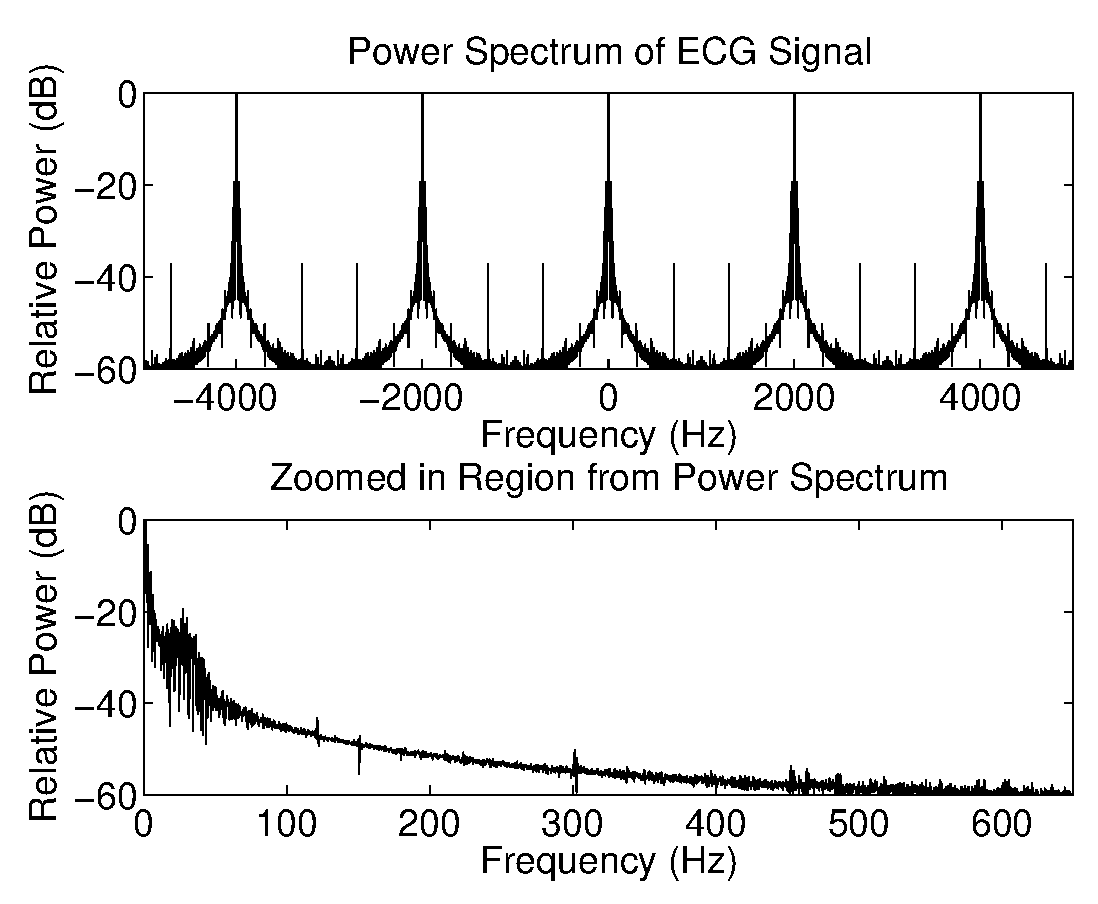
\includegraphics[width=3.0in]{ecg_sampling_fft.eps}
\end{center}

\begin{enumerate}
\item Based on the power spectrum above, what sampling rate (`XX') 
was used in the ADC?
\item What was the approximate Nyquist sampling rate for this signal?  How did
you determine this?
\item Sarah's friends go to Radio Shack buy her some op amps and resistors for
the task of building a DAC using a scaled resistor summing amplifier to convert
her saved ECG signal back to analog.  While thrilled with her birthday gifts,
she is disappointed that they didn't buy her any capacitors.  What would she
use a capacitor (or capacitors) to build, and why is that a necessary part of
the DAC process?
\item Design what is needed after the summing amplifier to complete her DAC and
restore the original, analog ECG signal.  (Be sure to follow the constraints
imposed by the power spectrum above!)
\item How many discrete digital signal levels can be represented with a 16-bit
binary number?  Given the specified SNR of the ECG signal (40 dB), are bits
being ``wasted'' sampling noise in this scenario?  What would be the ``ideal''
bit depth for this SNR?
\item Given a 90 bpm heart rate, if you were using a JK flip-flop-based counter
(like we covered in lecture and the problem sets) to count the number of beats
in the ECG over a 1 minute period, then how many JK flip flops would you need?
\end{enumerate}

\clearpage

{\bf BME154L - Exam \#1}\hfill Name:\underline{\hspace*{3.0in}}



\clearpage

{\bf BME154L - Exam \#1}\hfill Name:\underline{\hspace*{3.0in}}



\end{document}
